\section{Results}\label{sec:Results}

There are three grammars we analyze.%




\subsection{Parsing performance}

\begin{table*}[t]
%\begin{tabular}{p{.2\linewidth}| p{.18\linewidth} p{.18\linewidth}p{.18\linewidth}}
%&Maximal~Overlap, 1~vs.~Rest&Maximal~Overlap, Split&Shortest~Derivation, Split\\
\begin{tabular}{l | ccc}
&Maximal~Overlap&Maximal~Overlap&Shortest~Derivation\\
& 1~vs.~Rest& Split&Split\\\hline
labeled recall&90,97&90.14&84.90\\
labeled precision&90.25&90.10&84.39\\
labeled f-measure&90.61&90.12&84.64\\
exact match&53.27&49.53&39.25\\
leaf-ancestor&95.09&94.70&92.87\\
\end{tabular}

\caption{Results for 321 sentences of length$<16$}
\label{t:performance16}
\end{table*}

Table\ref{t:performance16} shows the parsing performance for the three grammars we constructed. Note that the POS-tags were passed to the parser in all cases, so tagging accuracy was 100\% and is omitted from this table. %Leaf-ancestor?



Both Maximal Overlap grammars perform much better than the Shortest Derivation one, in spite of the latter being consistent. 
One possible explanation, is the smoothing we conducted. Reall that the coverage of the Maximal Overlap approach is catered in a rather natural way, by extending the symbolic grammar with all PCFG rules from the treebank and treating them like the other fragments in the estimation. In the case of Shortest Derivation however, the coverage was a bit more artificial. $p_{unkn}$ was computed over all folds and used to redistribute weights over a classical PCFG constructed from the entire treebank. 

$p_{unkn}$ was found to be $1.41\times 10^{-3}$%0.00140590480016




\subsection{Pairwise comparison of the grammars}
In each plot, two grammars are compared to each other. The fragments are presented in a scatter plot, with the weights assigned by the two grammars along the axes. The weights are best visualized on a logarithmic scale. However, it is also informative to see those fragments with value zero. Therefore, the first interval ($[0,10^{-6}]$) is linear, while the rest of the plot is logarithmic. %symlog scaling

The difference between grammars is represented by the distance of the points to the \emph{identity} line ($x=y$).

The color corresponds to some feature, e.g. the depth of the fragment. The color mapping is also logarithmic. 


%Empirical results of our implementation (on the WSJ corpus?)
\paragraph{Comparing `split' to `one vs. rest'}
\begin{figure}
\center
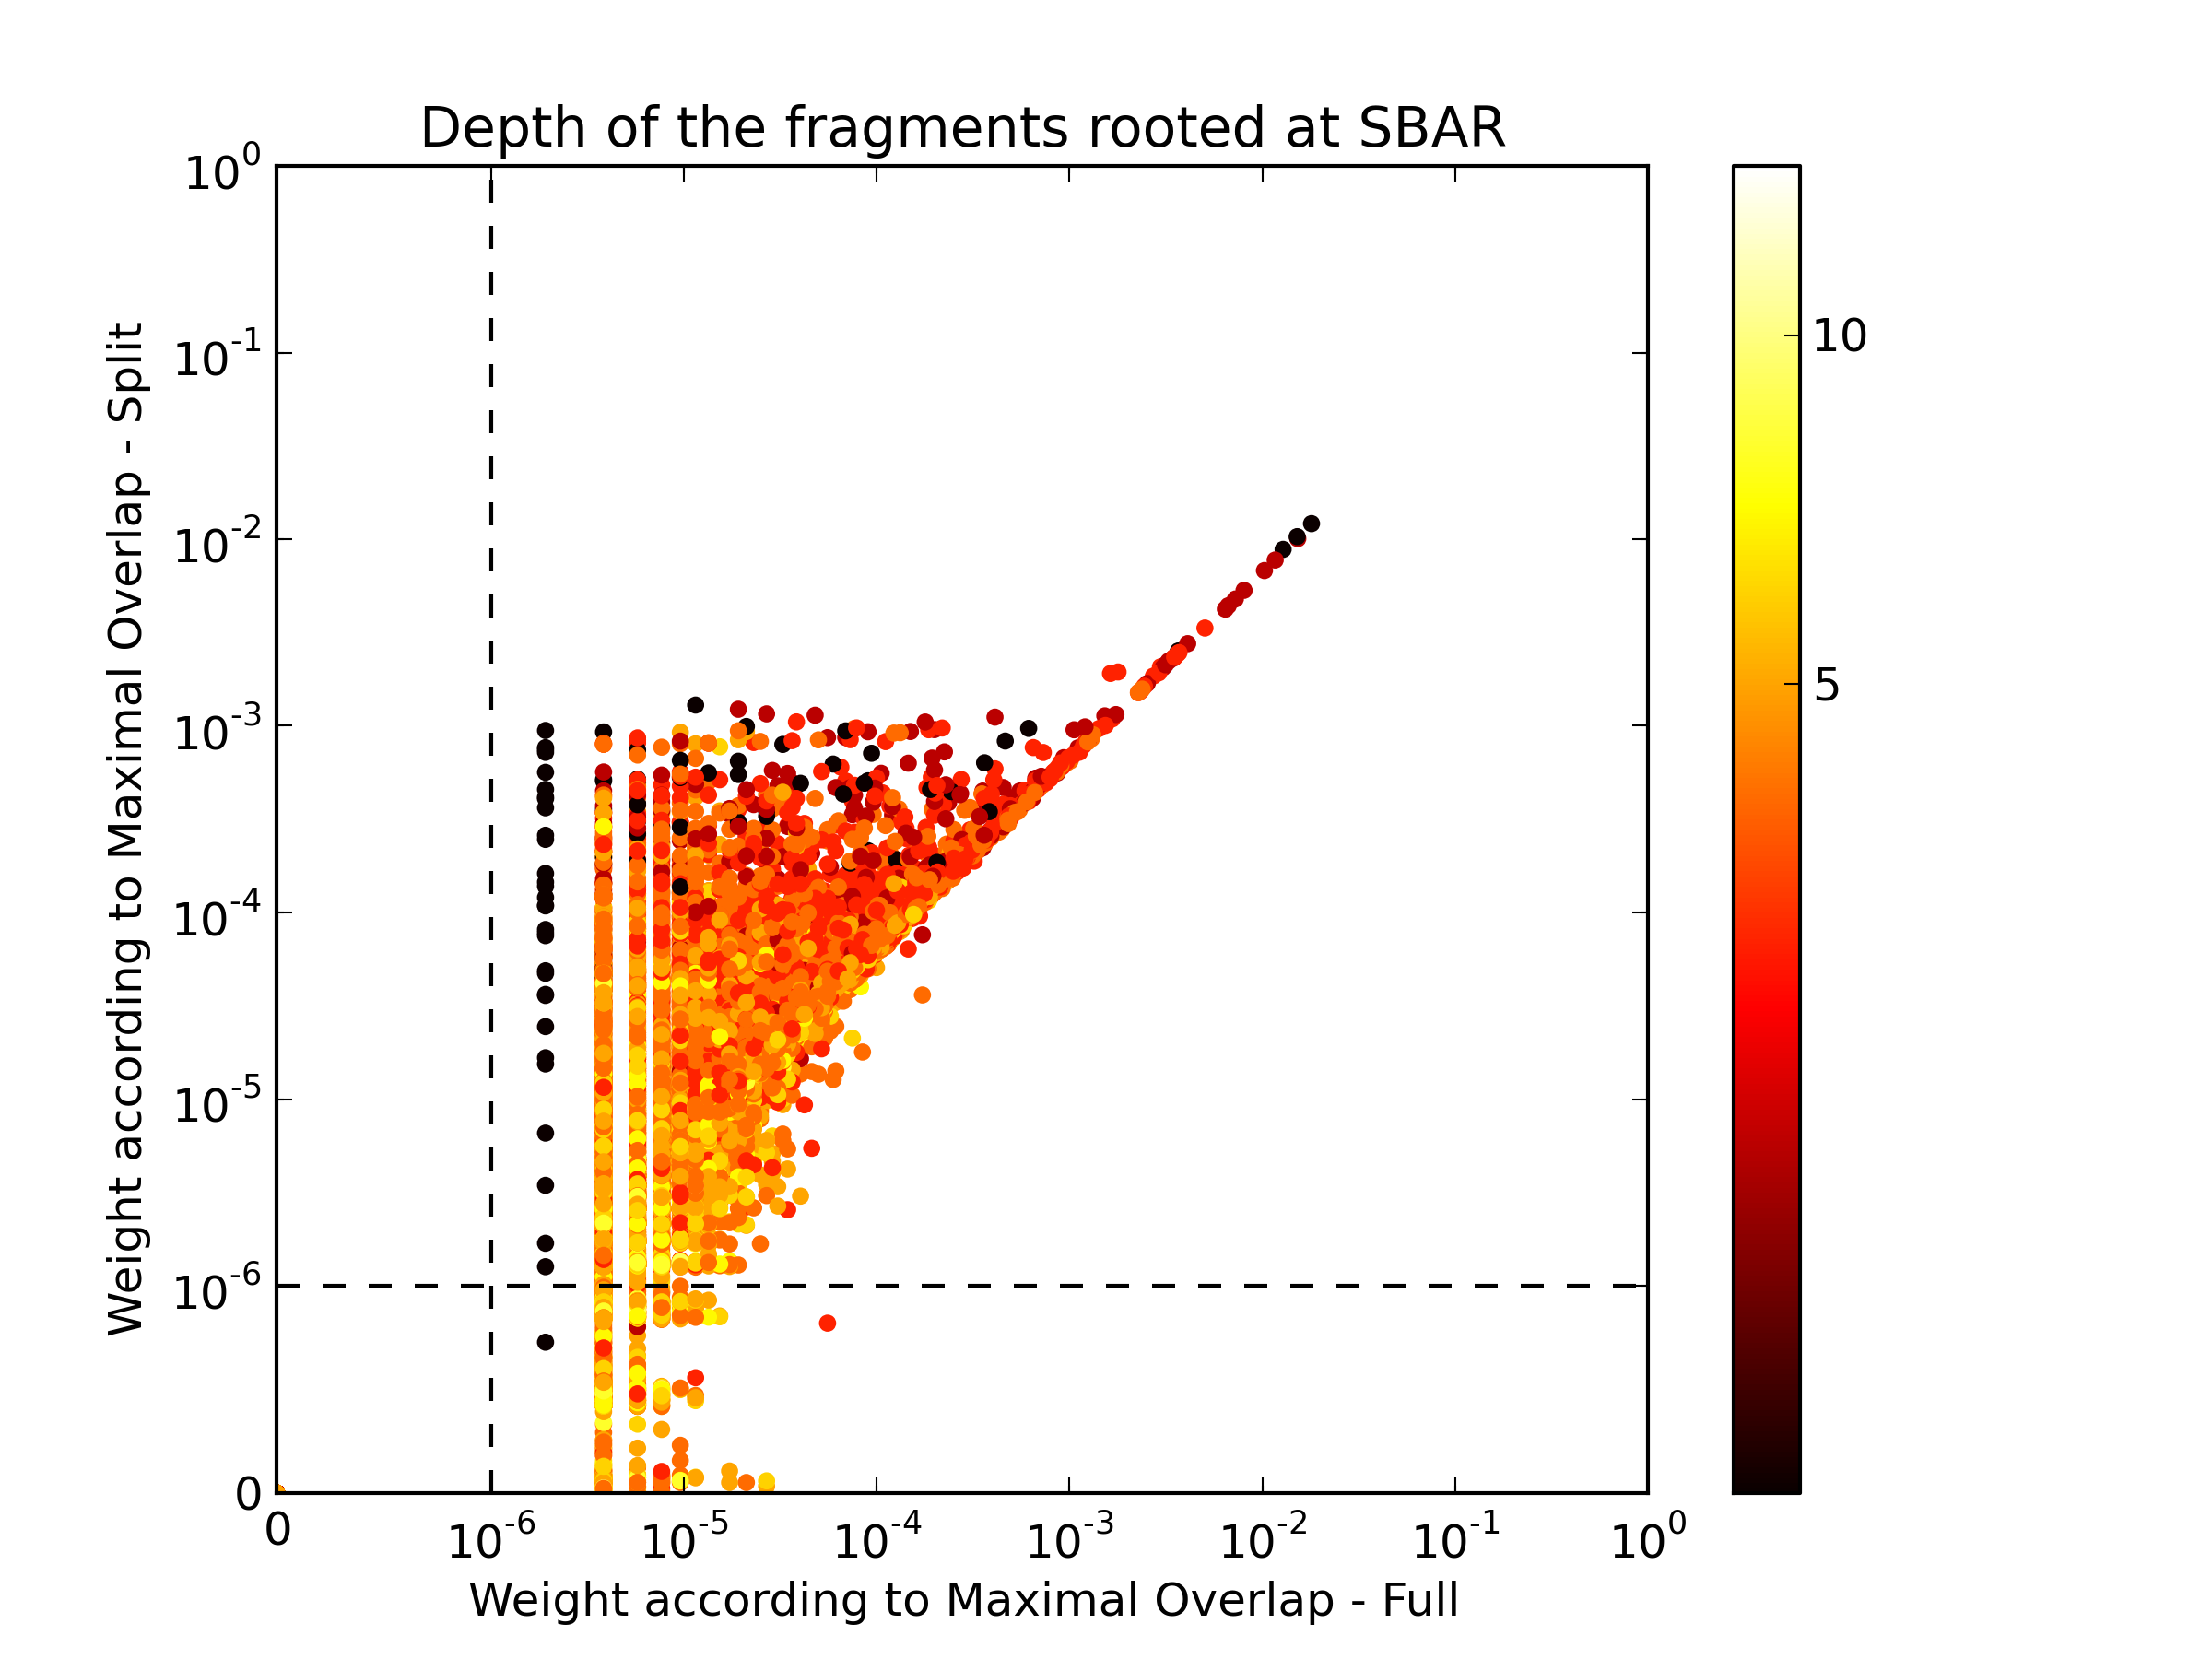
\includegraphics[width=\linewidth]{../data/plots/32.png}
\label{f:ddop-ddops-depth}
\end{figure}

Figure \ref{f:ddop-ddops-depth} illustrates the effect of the split estimation as compared to the one vs. rest. We see a remarkable separation of fragments with larger depth (lighter color) below the identity line, and fragments with smaller depth above it. This indicates that the split estimation tends to introduce a bias towards smaller fragments, or reduce the bias towards larger fragments.

%Diepe fragmenten zijn zwaarder in :
%	SD dan in MOS
%	SD dan MO
%	MO dan MOS (scherp)

%Brede fragmenten zijn zwaarder in:
% 	SD dan MOS (punt: CFG rules)
%	MO dan MOS (scherp)




























